\noindent
\begin{figure}[ht!]
  \centering
  \begin{subfigure}[t]{0.5\textwidth}
  	\centering
    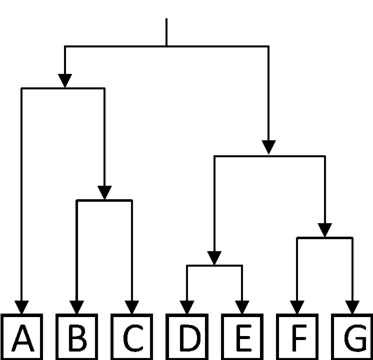
\includegraphics[width=0.40\textwidth]{hierarchical-clustering-example2}
	\caption{Hierarchical clustering example. The partial relation exists only between clusters.} \label{fig:hierarchical-example} 
  \end{subfigure}%
  ~
  \begin{subfigure}[t]{0.5\textwidth}
  	\centering
    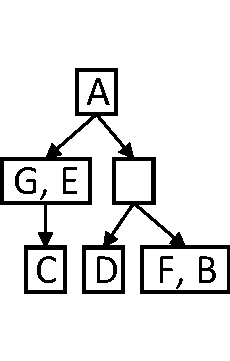
\includegraphics[width=0.40\textwidth, trim={0 1.15cm 0 1.15cm}, clip]{OCH-clustering-example}
	\caption{Object Cluster hierarchy example. The partial relation exists between both the clusters and the objects.} \label{fig:och-example} 
  \end{subfigure}
  \caption{Dendrogram and Object Cluster Hierarchy examples. Letters represent objects and squares are groups. The arrows show the partial order relation.}
\end{figure}